\documentclass{article}
\usepackage{geometry}
\usepackage{enumitem}
\usepackage{hyperref}
\usepackage{graphicx}

\hypersetup{colorlinks=true, linkcolor=black}


\geometry{a4paper, margin=1in}

\begin{document}

  \title{Content Delivery Network Design}
  \author{Bruno Zizi}
  \date{\today}

  \maketitle

  \tableofcontents

  \newpage

  \section{Introduction}
  This document outlines the design of a Content Delivery Network (CDN) for the storage and retrieval of images through
  HTTP.
  Trying to adhere as much as possible to the specified requirements, the proposed solution aims to address the
  challenge of creating a distributed system within an on-premise infrastructure emphasizing speed, robustness,
  security, scalability, and maintainability.


  \subsection{Preliminary Considerations and Assumptions}
  \begin{itemize}
    \item We value consistency more than latency in this implementation. We accept being slow in startup
     and during the Spread Procedure, but we can (almost) always sure that if an image is uploaded to the CDN, it
     will be available to all nodes.
    \item There is no one-size-fits-all solution. The implementation could be optimized in multiple ways.
    \item Granting a certain level of performance, always require a tailored solution. However multiple parameters
     are missing, such as the size of the CDN, expected traffic, security constraints (public vs. private), and so on.
  \end{itemize}


%  Objective section
  \section{Objectives}

  In this section of the document, we list a set of well-defined key objectives that would lead to an optimal solution
  for our CDN. These objectives guide the design and implementation of the CDN,
  ensuring that the solution is well-rounded, performs optimally, and meets the specified requirements.

  \begin{enumerate}[label=\arabic*.]
    \item \textbf{Speed:} Enable fast serving of content while also granting a fast and reliable spreading of newly
    uploaded images to all nodes in the network.

    \item \textbf{Robustness:} Implement a resilient system that can withstand node failures and recover quickly.

    \item \textbf{Security:} Mitigate DDoS attacks by consolidating Edge nodes behind a single IP using GBP protocol.
    Having a WAF in front of the Master nodes would also improve the overall security.

    \item \textbf{Scalability:} Design the CDN to efficiently handle an increasing number of nodes and images.

    \item \textbf{Maintainability:} Create a system that is easy to manage, ensuring the smooth operation of image
    storage and delivery.

    \item \textbf{Availability:} Enable Edge nodes to efficiently serve images even if not yet synchronized locally.

    \item \textbf{P2P Image Spreading:} Implement a P2P spreading mechanism for image distribution.

    \item \textbf{Master Node Coordination:} Utilize Master nodes to coordinate image spreading, maintain image records,
    and perform health checks on nodes.

    \item \textbf{Efficient Initial Synchronization (Edge node bootstrap):} Facilitate quick initial synchronization
    for Edge nodes joining the network.

    \item \textbf{Edge Node Caching:} Leverage caching mechanisms whenever possible  for improved performance.
  \end{enumerate}





  \newpage







  \section{Network Topology}
  The CDN is designed as a distributed system within an on-premise infrastructure.
  The topology involves multiple interconnected nodes each serving a specific purpose.
  Below is an overview of the key components and their relationships:

  \subsection{Master Nodes}
  Master Nodes play a central role in coordinating the CDN network.
  They maintain a comprehensive record of available images, orchestrate image spreading procedures,
  and perform health checks on connected Edge Nodes. The Master Nodes ensure the consistency and reliability of the CDN.


  \subsection{Edge Nodes}
  Edge Nodes act as the gateways for handling incoming HTTP requests and serving images.
  These nodes are distributed strategically to optimize content delivery and reduce latency.
  Each Edge Node communicates with the Master Node for synchronization and image spreading.
  From a very high level standpoint, they can be considered as some sort of Master Nodes distributed cache.

  \subsection{DNS (Load Balancer)}
  DNS nodes are responsible for directing incoming HTTP requests to the appropriate Edge Node.
  These components enhance the overall system's scalability, security and performance by efficiently
  distributing the incoming traffic.

  \subsection{WAF (Web Application Firewall)}
  The WAF adds an additional layer of security to the CDN infrastructure.
  Placed in front of the Master Nodes, it helps mitigate potential security threats,
  including Distributed Denial of Service (DDoS) attacks, thus ensuring availability.

  \subsection{Internal messaging system}
  Utilizing fast and asynchronous messaging systems such as RabbitMQ or Kafka could mitigate
  communication costs between nodes. This is achieved by minimizing the reliance on HTTP over TCP connections
  wherever possible.

  \subsection{CDN Internal Network}
  The CDN Internal Network comprises the interconnected Edge Nodes, Master Nodes, Load Balancer, and WAF.
  This internal network ensures secure communication and data transfer among CDN components
  while isolating them from the public internet.


  \begin{figure}
    \centering
    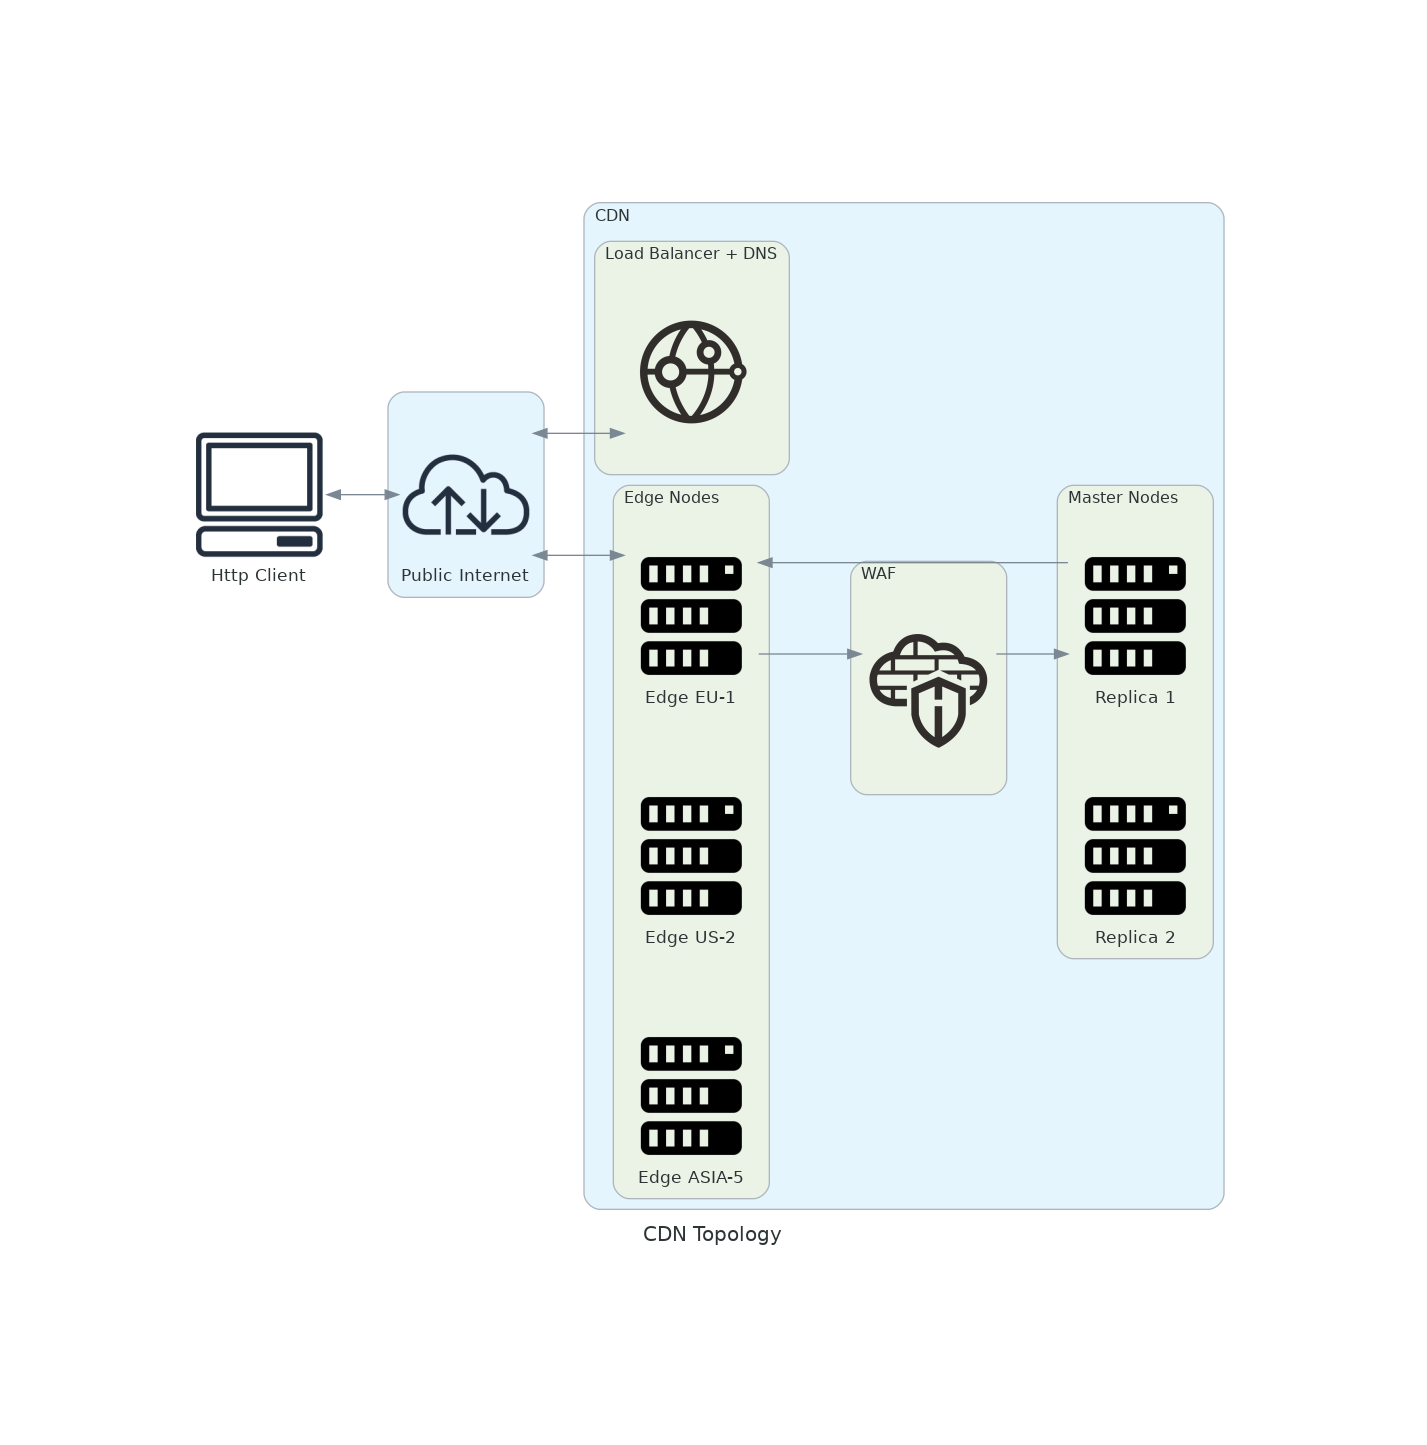
\includegraphics[width=1.0\textwidth]{imgs/cdn_topology}
    \caption{CDN Topology}
    \label{fig:cdn topology}
  \end{figure}






  \newpage







%  section main flows
  \section{Main Flows}

  \subsection{Bootstrap Procedure}

  \textit{Description:} The Bootstrap Procedure is initiated when an Edge Node joins the network for the first time or
  restarts after being down. Its purpose is to synchronize the new or recovering node with the existing network,
  ensuring it has the necessary information to serve images.

  \textit{Implementation:} The Edge Node communicates with the Master Node to obtain a list of available images
  and the next node(s) from which it should download images.

  \textit{Flow:}
  \begin{enumerate}[label=\arabic*.]
    \item When an Edge Node needs to bootstrap (either because it's joining the network for the first time or
    restarting after downtime), it sends a bootstrap request to the Master Node.

    \item Upon receiving the bootstrap request, the Master Node responds with a map of available images and the
    corresponding IP addresses of nodes from which the images can be downloaded. If the bootstrap request
    contains a starting date, indicating a specific date from which the Edge Node needs
    images, only images updated after that date will be included.

    \item The Edge Node, upon receiving the response from the Master Node, starts the process of
    downloading the images indicated in the map.
    To optimize the procedure, a 'batch download' operation could
    be implemented.

    \item The Edge Node may also initiate a spread procedure to receive any new images uploaded to the
    network during its downtime.

    \item Once the Bootstrap Procedure is complete, the Edge Node is synchronized with the network and can
    efficiently serve images to end-users.
  \end{enumerate}

 \newpage

  \begin{figure}
    \centering
    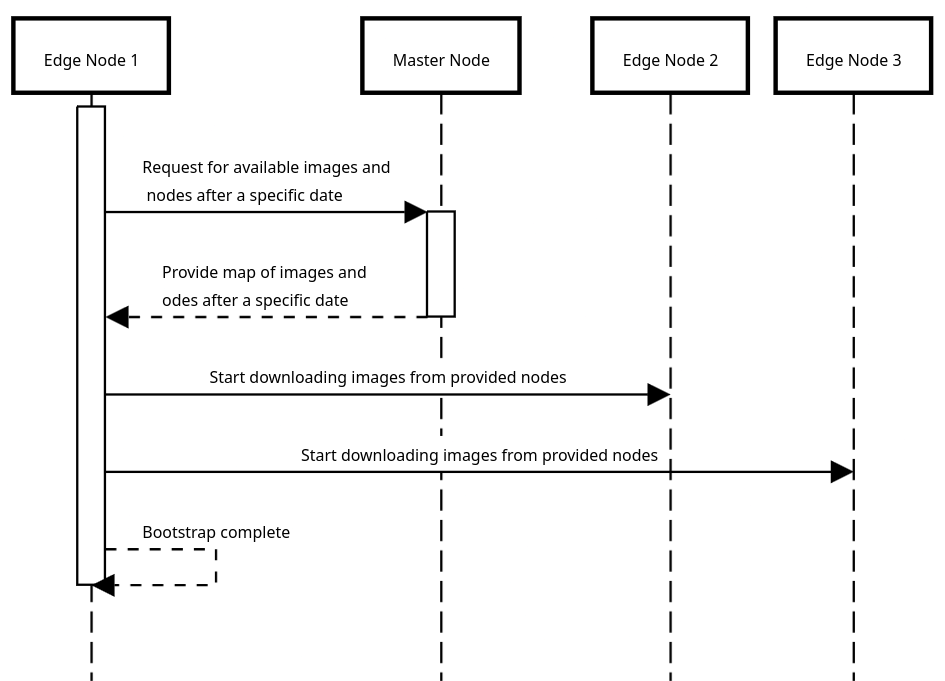
\includegraphics[width=1.0\textwidth]{imgs/bootstrap_procedure}
    \caption{Bootstrap procedure}
    \label{fig:Edge node bootstrap procedure}
  \end{figure}







  \newpage







  \subsection{Image Spreading Procedure}

  \textit{Description:} The Image Spread Procedure is initiated when a new image is uploaded to the network. Its
  purpose is to efficiently distribute the newly uploaded image to all connected Edge Nodes, ensuring quick
  availability for end-users.

  \textit{Implementation:} The Edge Node, upon receiving a new image upload request, notifies the Master Node about
  the new image. The Master Node, in turn, determines the next connected Edge Node(s) to which the image
  should be pushed for spreading.

  \textit{Flow:}
  \begin{enumerate}[label=\arabic*.]
    \item When a new image is uploaded, the Edge Node receiving the upload request adds the image to its
    list of available images and saves it locally.

    \item The Edge Node notifies the Master Node about the new image upload, providing relevant details such
     as image metadata.

    \item Upon receiving the notification, the Master Node updates its records to include the newly
    uploaded image in its list of available images.

    \item The Master Node determines the next connected Edge Node(s) in the spreading sequence.
    This could be based on factors like load balancing, geographic proximity, or any defined distribution strategy.

    \item The Master Node replies to the uploading Edge Node with the IP address(es) of the next node(s)
    in the spreading sequence.

    \item The Edge node pushes the image to the next node.
  \end{enumerate}


  \begin{figure}
    \centering
    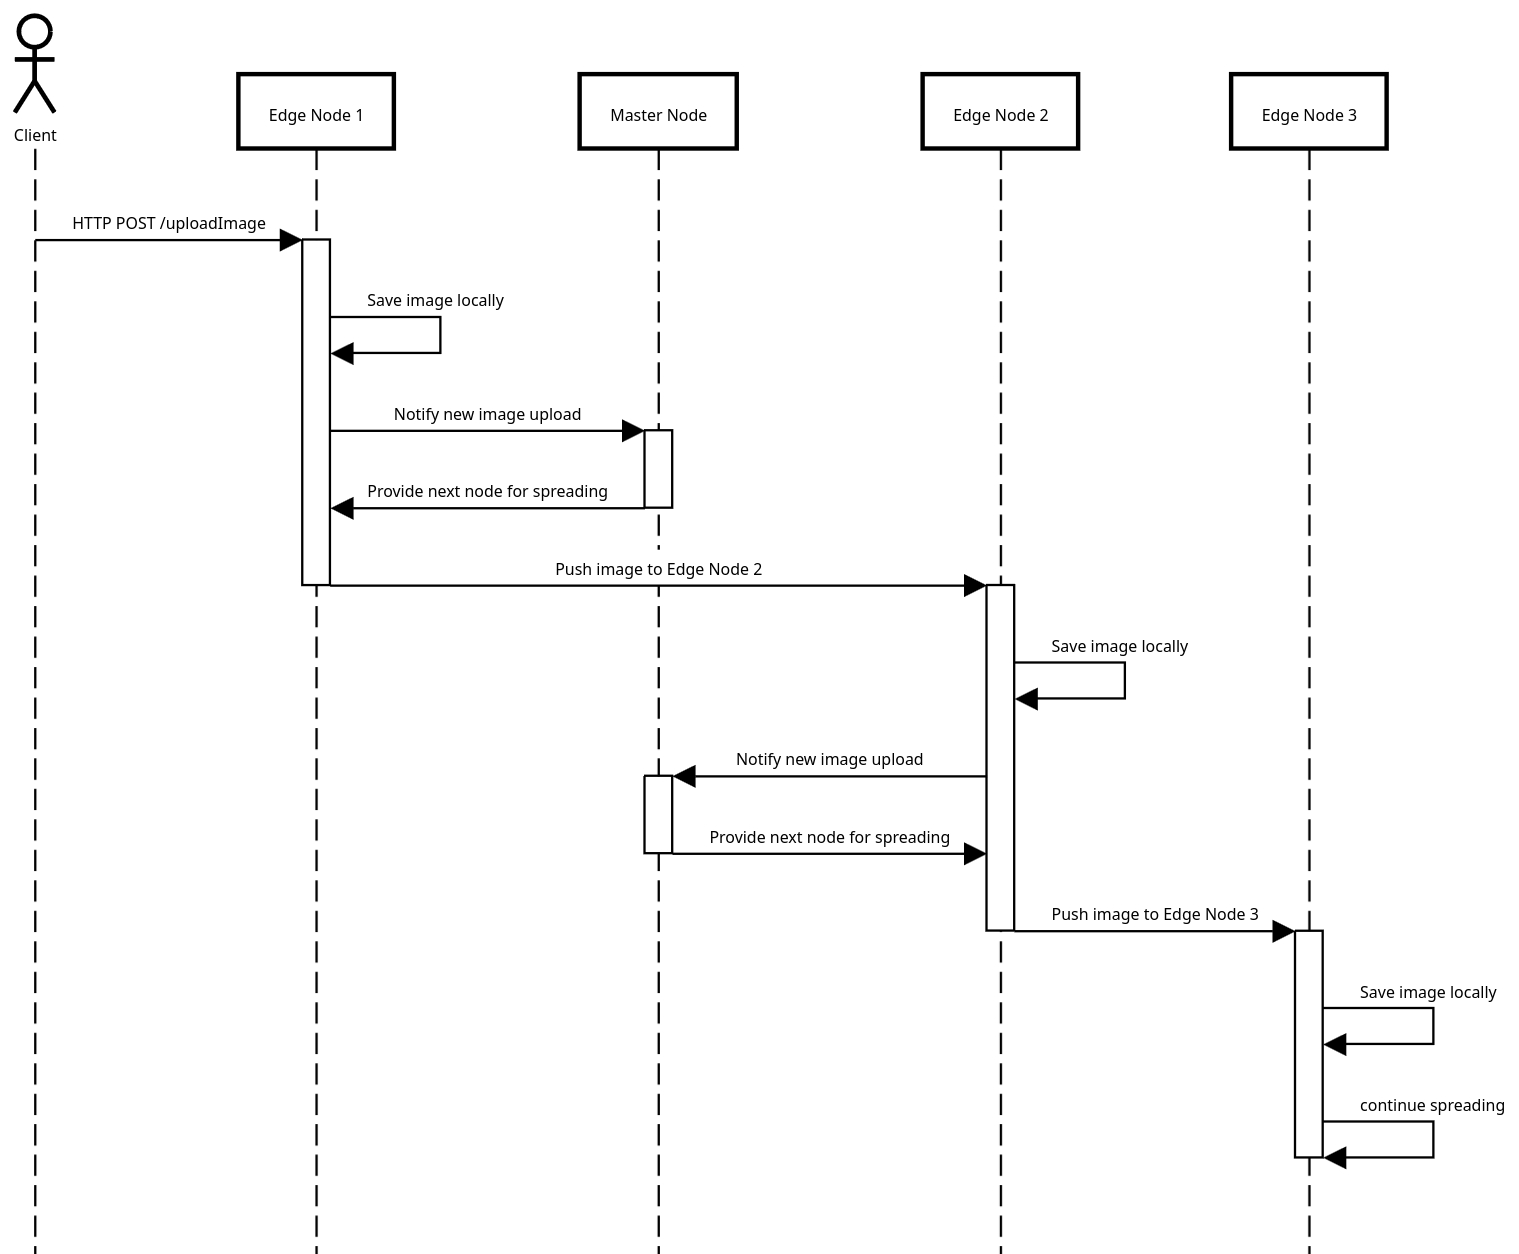
\includegraphics[width=1.0\textwidth]{imgs/spread_procedure}
    \caption{Image spreading procedure}
    \label{fig:Image spreading procedure}
  \end{figure}




  \newpage






  \section{Edge node implementation}

  \subsection{Communication with Master Node}
  \textit{Description:} Communicate with the Master Node for initial setup and the spread procedure.

  \textit{Implementation:} Use HTTP requests or a messaging system like Kafka or RabbitMQ for communication.

  \textit{Flow:}
  \begin{enumerate}[label=\arabic*.]
    \item Upon initialization, request the list of available images from the Master Node.
    \item Utilize the spread procedure to receive all new images from the Master Node when they are uploaded.
    \item If the node goes down and restarts, initiate a synchronization process with the Master Node.
  \end{enumerate}



  \subsection{Bootstrap Procedure}
  \textit{Description:} Procedure for an Edge Node to join the network for the first time or after being down.

  \textit{Implementation:} Check with the Master Node for the list of available images and nodes for image downloading.

  \textit{Flow:}
  \begin{enumerate}[label=\arabic*.]
    \item When an Edge Node initiates a bootstrap request, the Master Node receives the request.
    \item The Master Node responds with a map of available images and the corresponding IP addresses of nodes
    from which the images can be downloaded. If the bootstrap request includes a starting date, the Master Node tailors
    the map to contain onlyi mages updated after that specific date. This is usefull in case of downtime recovery.
    \item The Edge Node, upon receiving the response from the Master Node, starts downloading all the images
    indicated in the map.
  \end{enumerate}


  \subsection{Caching Mechanism}
  \textit{Description:} Cache frequently accessed images locally for improved retrieval speed.

  \textit{Implementation:} Utilize a caching system like Redis or Memcached.

  \textit{Flow:}
  \begin{enumerate}[label=\arabic*.]
    \item Upon receiving an HTTP request, check the local cache for the requested image.
    \item If the image is present and not expired, serve it directly.
    \item If the image is not in the cache or has expired, fetch it from the Master Node and update the cache.
  \end{enumerate}


  \subsection{Logging and Tracing}
  \textit{Description:} Record and trace relevant events for monitoring and debugging.

  \textit{Implementation:} Use a logging library and incorporate distributed tracing (e.g., OpenTelemetry).

  \textit{Flow:}
  \begin{enumerate}[label=\arabic*.]
    \item Log key events such as incoming requests, cache hits/misses, interactions with the Master Node and errors as well.
  \end{enumerate}


  \subsection{Health Check}
  \textit{Description:} Regularly check the health of the Edge Node.

  \textit{Implementation:} Implement a health-check mechanism and leverage the Master Node's health-check capabilities.

  \textit{Flow:}
  \begin{enumerate}[label=\arabic*.]
    \item Expose an HTTP endpoint for health checks or use a dedicated Kafka topic.
    \item Alternatively, an Edge Node could periodically ping the Master Node to report its health status.
  \end{enumerate}


  \subsection{Additional Considerations}

  \textit{Implementation:}
  \begin{itemize}
    \item Implement a configuration mechanism to adjust parameters such as cache expiration times and synchronization
    intervals.
    \item Employ exponential backoff strategies for retries during communication with the Master Node to handle
    potential network issues.
  \end{itemize}






  \begin{figure}
    \centering
    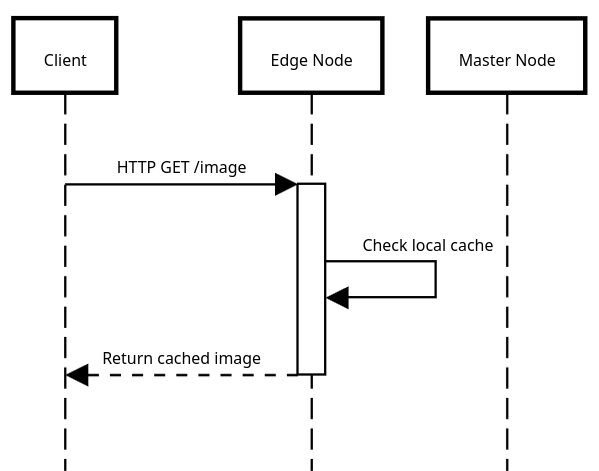
\includegraphics[width=1.0\textwidth]{imgs/cache_hit}
    \caption{Edge node cache hit}
    \label{fig:Edge Node - cache hit scenario}
  \end{figure}




  \begin{figure}
    \centering
    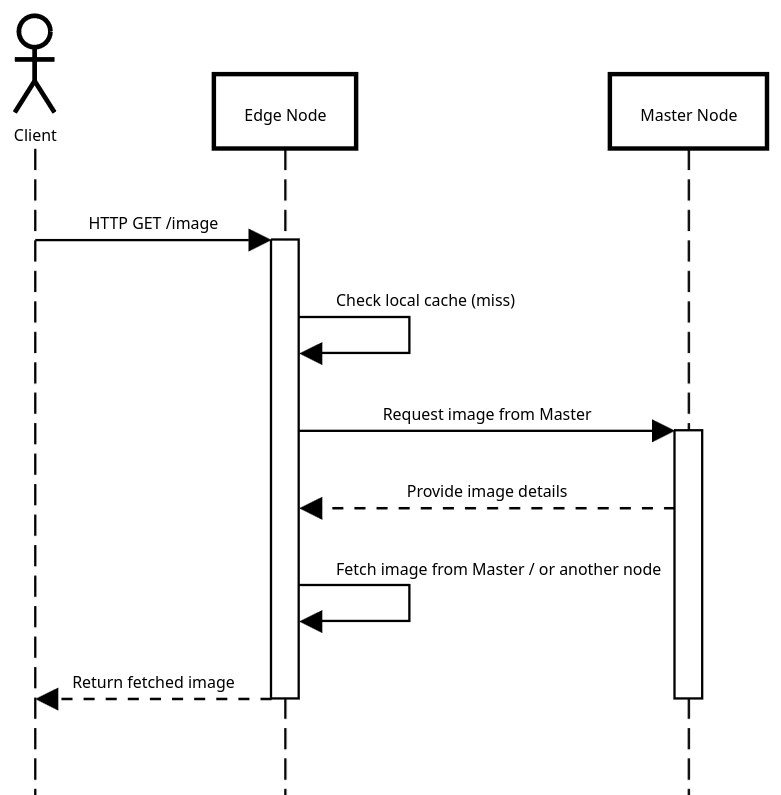
\includegraphics[width=1.0\textwidth]{imgs/cache_miss}
    \caption{Edge cache miss}
    \label{fig:Edge Node - cache miss scenario}
  \end{figure}







  \newpage









  \section{Master Node Implementation}

  \subsection{Handling HTTP Requests}

  \textit{Description:} Receive incoming HTTP requests for various operations (e.g., image spreading, health checks).

  \textit{Implementation:} Utilize a robust HTTP server library in C++ or Go.

  \textit{Flow:}
  \begin{enumerate}[label=\arabic*.]
    \item Listen for incoming HTTP requests.

    \item Route requests based on operation types (spread, health check, etc.).

    \item Handle each type of request accordingly.
  \end{enumerate}



  \subsection{Image Spreading Procedure}

  \textit{Description:} Distribute newly uploaded images to all connected Edge Nodes.

  \textit{Implementation:} Utilize a push-based mechanism and reply with the IP(s) of the next node for spreading.

  \textit{Flow:}
  \begin{enumerate}[label=\arabic*.]
    \item Receive a new image upload request.

    \item Add the image to the list of available images and save it locally.

    \item Identify connected Edge Nodes that haven't already received the image.

    \item Reply with the IP(s) of the next Edge Node(s) for spreading.
  \end{enumerate}


  \subsection{Bootstrap Procedure (Master Node)}

  \textit{Description:} Procedure for an Edge Node to join the network for the first time or after being down.

  \textit{Implementation:} Check with the Master Node for the list of available images and nodes for image downloading.

  \textit{Flow:}
  \begin{enumerate}[label=\arabic*.]
    \item When an Edge Node needs to bootstrap (either because it's joining the network for the first time or
    restarting after downtime), it sends a bootstrap request to the Master Node.

    \item Upon receiving the bootstrap request, the Master Node responds with a map of available images and the
    corresponding IP addresses of nodes from which the images can be downloaded. If the bootstrap request
    contains a starting date, indicating a specific date from which the Edge Node needs
    images, only images updated after that date will be included.

    \item The Edge Node, upon receiving the response from the Master Node, starts the process of
    downloading the images indicated in the map.
    To optimize the procedure, a 'batch download' operation could be implemented.

    \item The Edge Node may also initiate a spread procedure to receive any new images uploaded to the
    network during its downtime.

    \item Once the Bootstrap Procedure is complete, the Edge Node is synchronized with the network and can
    efficiently serve images to end-users.
  \end{enumerate}



  \subsection{Maintaining Image Records}

  \textit{Description:} Keep track of all available images in the CDN.

  \textit{Implementation:} An in-memory data store or a database can be used for the purpose.

  \textit{Flow:}
  \begin{enumerate}[label=\arabic*.]
    \item Maintain a data structure to store image metadata (e.g., filename, ID, timestamp).

    \item Update the record upon each image upload.
  \end{enumerate}



  \subsection{Health Check Mechanism}

  \textit{Description:} Receive (and handle) health checks data from connected Edge Nodes.

  \textit{Implementation:} Handle health-check requests from Edge Nodes. It can be implemented as a synchronous (HTTP)
  or an asynchronous  (message queue) operation.

  \textit{Flow:}
  \begin{enumerate}[label=\arabic*.]
    \item Receive health checks data from connected Edge Nodes.

    \item Update the health status for requesting nodes.
  \end{enumerate}



  \subsection{Logging and Tracing}

  \textit{Description:} Record and trace relevant events for monitoring and debugging.

  \textit{Implementation:} Use a logging library and incorporate distributed tracing (e.g., OpenTelemetry).

  \textit{Flow:}
  \begin{enumerate}[label=\arabic*.]
    \item Log key events such as incoming requests, image spreading, health-check results as well as errors.
  \end{enumerate}









  \newpage







  \section{Conclusion}

  The designed CDN presents a comprehensive solution to the initial
  requirements, emphasizing consistency, speed, robustness, security, and scalability.
  However like any system, there are considerations regarding potential weak points and areas for improvement.

  \subsection{Consistency vs. Latency Trade-off}
  The chosen approach prioritizes consistency over latency during startup and image spreading procedures.
  This decision may result in slower initial synchronization and image spreading but guarantees that uploaded
  images are eventually available on all nodes. For scenarios where low-latency is critical,
  optimizing the trade-off may be explored based on specific use-case requirements.

  \subsection{Tailored Optimization}
  The design recognizes that there is no one-size-fits-all solution. Various parameters,
  such as CDN size, expected traffic, and security constraints, are missing or assumed.
  Tailoring the implementation based on these parameters could lead to further adjustments and optimization.

  \subsection{Peer-to-Peer Communication}
  While peer-to-peer communication enhances image spreading efficiency,
  challenges may arise in ensuring secure and reliable communication between Edge Nodes.
  Implementing robust mechanisms for peer discovery, authentication, and data integrity is
  essential to mitigate potential risks associated with peer-to-peer communication.

  \subsection{Distributed Configuration}
  One notable weak point in the current design is the lack of detailed considerations for a
  distributed configuration management system. As the CDN dinamically scales and grows, the need for
  an efficient configuration updates becomes crucial. Implementing a robust distributed configuration
  management system can enhance the flexibility and reduce the time to market significantly.

  \subsection{Service Discovery}
  Another area that requires attention is service discovery. The current design assumes a relatively
  static environment with predefined IP addresses for communication between nodes.
  In dynamic and large-scale deployments, a robust service discovery mechanism is essential to automatically
  locate and connect to nodes.




\end{document}
